
\documentclass[11pt]{article}

\marginparwidth 0.2in 
\oddsidemargin 0.1in 
\evensidemargin 0.1in 
\marginparsep 0.1in
\topmargin 0.1in 
\textwidth 6.5in \textheight 8 in

\usepackage{hyperref}  
\usepackage{listings}
\usepackage{array}
\usepackage{multirow}
\usepackage{attachfile}
\usepackage{lscape}
\usepackage{graphicx}

\begin{document}

\author{İbrahim Burak Tanrıkulu, 21827852}
\title{BBM436 Microprocessors Lab.\\Assignment 7\\Communication with peripherals}
\maketitle

\section{Communication Styles}
Communication is transfer or reception of electromagnetic signals over wires, optical fibers or wireless communication channels. Microprocessors use parallel or serial communication over wire/s.\\

{\bf Parallel Communication: }\\
Parallel communication is a method of conveying multiple binary digits (bits) simultaneously. Microprocessors have address and/or data pins for parallel communication. Number of these pins determine width of data transfer. For example, 8086 mP have 16 data pins. This means that this microprocessor can transmit or receive 2 bytes of data simultaneously.\\

{\bf Serial Communications: }\\
Serial communication is the process of sending data one bit at a time, sequentially, over one wire. For transmitting or receiving data, microprocessors can use software (for example, bit banging) or hardware (USART). Serial communication can be synchronous or asynchronous.\\

{\bf Asynchronous:} In this communication style, we use start bit, parity bit and stop bit. If we are not transferring data, signal will be in a idle state(high voltage). Start(0) and stop(1) bit are mandatory, parity bit is optional. Parity bit is used for validity of transfer. Also, transmitter and receiver devices must use same baud rate, which means how many bits will transfered in 1 second. We use UART hardware for converting parallel data to serial data.\\

{\bf Synchronous:} In this communication style, we use clock signal. Data is sent in a continuous stream according to clock signal. Also, no start or stop bits are needed in this communication. But still we use control bytes to specify start or stop. There are different protocols in synchronous communication. Some protocols use ASCII characters, some of them use four-of-eight codes, some of them use bits.\\

{\bf Bit-oriented synchronous protocols:} Bit-oriented protocols transmit data as a stream of bits with no semantics or meaning. Control codes are defined in terms of bit sequences. Synchronization is maintained on an idle line by transmitting a predefined sequence of bits. Synchronous Data Link Control (SDLC) was the first bit-oriented protocol developed. It was later adopted by ISO as High-Level Data Link Control (HDLC). Logical Link Control (LLC) and Advanced Data Communication Control Procedures (ADCCP) are other examples of bit-oriented protocols.

{\bf Byte-oriented synchronous protocols:} In this protocol, we transferring data byte-by-byte. For synchronization, certain number of idles were sent prior to each transmission. The IBM Binary Synchronous protocol (Bisync) is still in use, Other examples of byte-oriented protocols are IBM's Synchronous transmit-receive (STR), and Digital Data Communications Message Protocol (DDCMP) from Digital Equipment Corporation. 

\section{Proteus applications}
{\bf Asynchronous communication between two 8086 microprocessors}\\
In this part, i used bit banging for transmitting data. Microprocessors and virtual terminals will be run on 9600 baud rate, no parity bit, 8 data bit and 1 stop bit. Used d flip-flop for constant signal. IN and OUT instructions make signals momentary. Thus reading a signal is easier with this d flip-flop. When slave microprocessor receives one byte, master microprocessors waits and slave microprocessor prints the data to virtual terminal. \ref{asenkron} Project File: \attachfile{Async.pdsprj}

{\bf Synchronous communication between two 8086 microprocessors}\\
In this part, i used Bisync protocol. An example frame of Bisync is:\\
\begin{tabular} {|c|c| c| c| c| c| c| c| }
 \hline
 SYN & SYN & SOH & Header & STX & Text & ETX & CRC \\
\hline
\end{tabular}\\
Master microprocessor sends these control and text bytes. Slave microprocessor controls the order of frame; if it is right, pushes text bytes into a stack. When transmission is complete, pops these text bytes from stack and sends to virtual terminal asynchronously. \ref{senkron} Project File: \attachfile{Bisync.pdsprj}
\section{Comparative table}
\begin{tabular}{|l|c|c|c|c|}
\hline
 & Parallel & \multicolumn{3}{c|}{Serial}\\
\hline
Speed & Fast, dependent to \# of pins & \multicolumn{3}{c|}{Slower}\\
\hline
Space & Lots of cables & \multicolumn{3}{c|}{a few cables}\\
\hline
Complexity & Easy & \multicolumn{3}{c|}{Need to converted by USART}\\
\hline
Crosstalk & More & \multicolumn{3}{c|}{Less}\\
\hline
Usege & computer BUSes & \multicolumn{3}{c|}{Peripherals, telecommunication}\\
\hline
&  & Asynchronous & \multicolumn{2}{c|}{Synchronous}\\
\hline
Need clock & Yes & No & \multicolumn{2}{c|}{Yes}\\
\hline
 & & & Bit-oriented & Byte-oriented \\
\hline
bits needed for a byte & 8 & 10$<$= & 24$<$= & 48$<$= \\
\hline
N byte message & N byte & 1.25 * N byte & 8*N + 32 & 8*N + 48 \\
\hline
\end{tabular}
\newpage
\begin{figure}[h!]
	\centering
	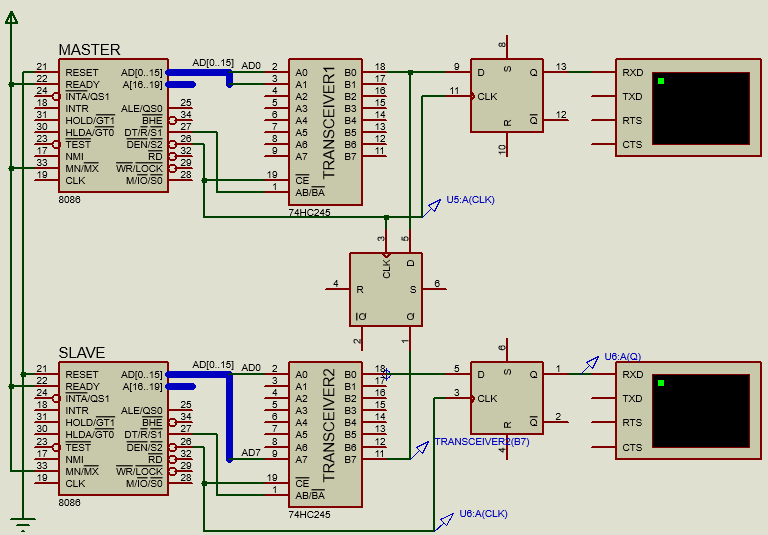
\includegraphics[width=12cm]{Asenkron.png}
	\caption{Asynchronous communication design}
	\label{asenkron}
\end{figure}

\begin{figure}[h!]
	\centering
	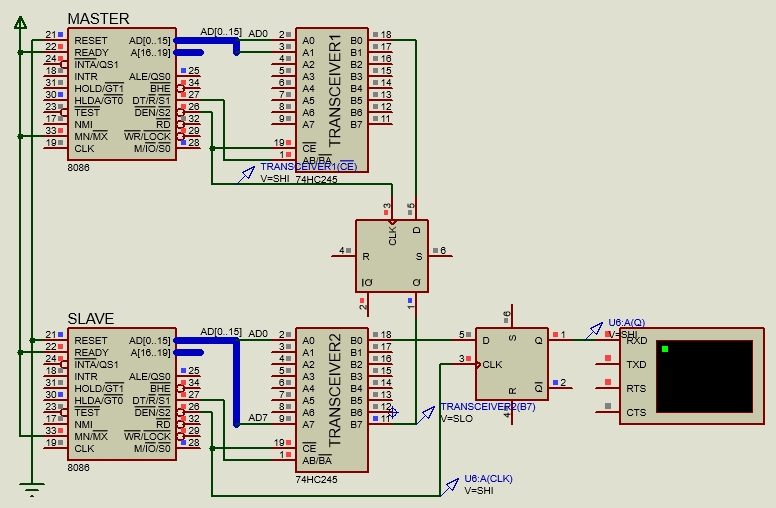
\includegraphics[width=12cm]{Senkron.png}
	\caption{Synchronous communication design}
	\label{senkron}
\end{figure}

\end{document}
